\section{Ring Signatures}
In a standard UTXO transaction the sender signs the transactions using his/her
private key and the signatory can be explicitly determined and identified. In
cryptography, \textbf{a ring signature} is a type of digital signature that can be
performed by any member of a defined group of users that each have the required
keys. A distinctive \textbf{ring signature} is produced through a process that combines
the keys of all possible signers and other values and which are then subject to
a hash function.



In cryptography a ring signature is a form of a \textit{non-interactive 
zero knowledge proof}\footnote{https://en.wikipedia.org/wiki/Non-interactive\_zero-knowledge\_proof}. 
In layman’s terms, what this means is simply that you can prove the
correctness of a statement/transaction to a verifier without leaking any additional
information by just using a shared common reference string (\textit{public key}).
This system must include cryptographic completeness, soundness and zero-knowledge.



\underline{Completeness} means that if the statement is correct, then the verifier will
always accept. \underline{Soundness} is a property of such a system that requires that
no prover can make the verifier accept a false or incorrect statement. If the
statement is incorrect or false, then the verifier will always reject. The
last part is \underline{zero knowledge}. It is not possible to gain any extra information
from the proof itself for any malicious verifier except for the correctness of
the statement.



This offers a group member a level of anonymity not attainable through generic
digital signature schemes. This is a property known as ‘\textit{plausible deniability}’,
or anonymity with respect to an anonymity set. With a ring size of 10 for example
there are 10 possible signatories, i.e. 10 public keys and an observer cannot
determine which one corresponds to the \textbf{SPECTRE} spent in the transaction. This
is only known to the sender. This protects the privacy of the sender. With every
transaction using a ring-signature the network ‘\textit{transactional entropy}’ increases
and it becomes increasingly hard to link input/output on the blockchain.



Look at it like this; scattered along the Spectrecoin blockchain are ATXOs of
various denominations from 1000 to 0.00000001 SPECTRE. These ATXOs may be spent
or unspent but this cannot be determined by an observer. The proof of an ATXO
being spent is formed on an ad-hoc basis through the creation of a ‘\textit{keyimage}’
and there is nothing contained within the data of the ATXO itself or the
transaction data written to the blockchain that signifies if it has ever been
‘\textit{spent}’. In a standard UTXO transaction on the other hand an observer can
explicitly determine that an UTXO has indeed been spent to create a new UTXO.



See the illustrations on the next page to visualise the difference between an
UTXO and ATXO.



\subsection{Standard UTXO transaction}

\begin{figure}[h]
	\caption{Standard UTXO transaction}
	\centering
	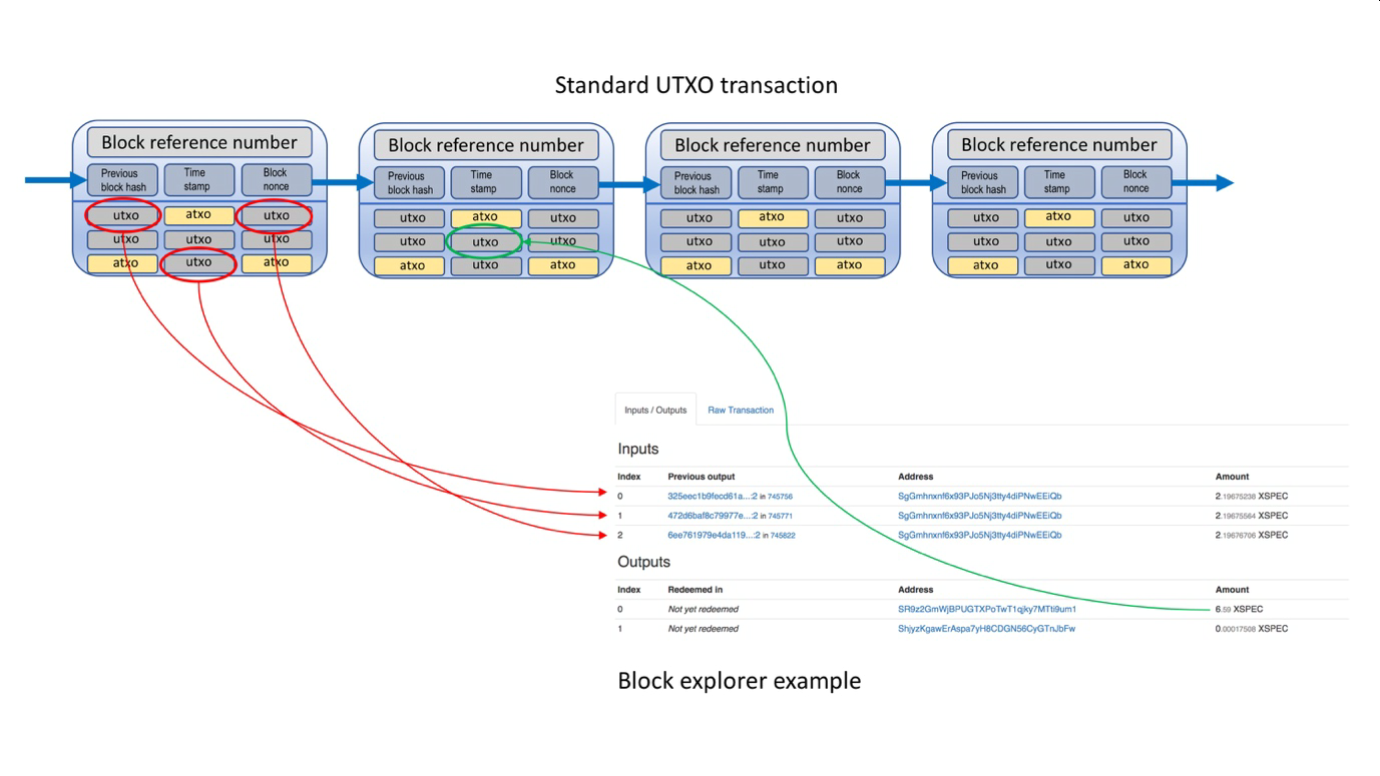
\includegraphics[width=\textwidth]{Std-UTXO-Transaction.png}
\end{figure}



On the blockchain there is a \textbf{\underline{direct}} correlation
between the inputs and the outputs, and all the transactions can be 
traced back to the genesis transactions. This is still the case even 
if a mixing strategy is used, such as in DASH. There are increasingly 
sophisticated methods to analyse blockchain data and this is a growth 
industry. You should consider any standard UTXO transactions to be 
non-anonymous and public, whether with Spectrecoin or Bitcoin.



\subsection{Anonymous ATXO transaction}



\begin{figure}[h]
	\caption{SPECTRE ATXO transaction}
	\centering
	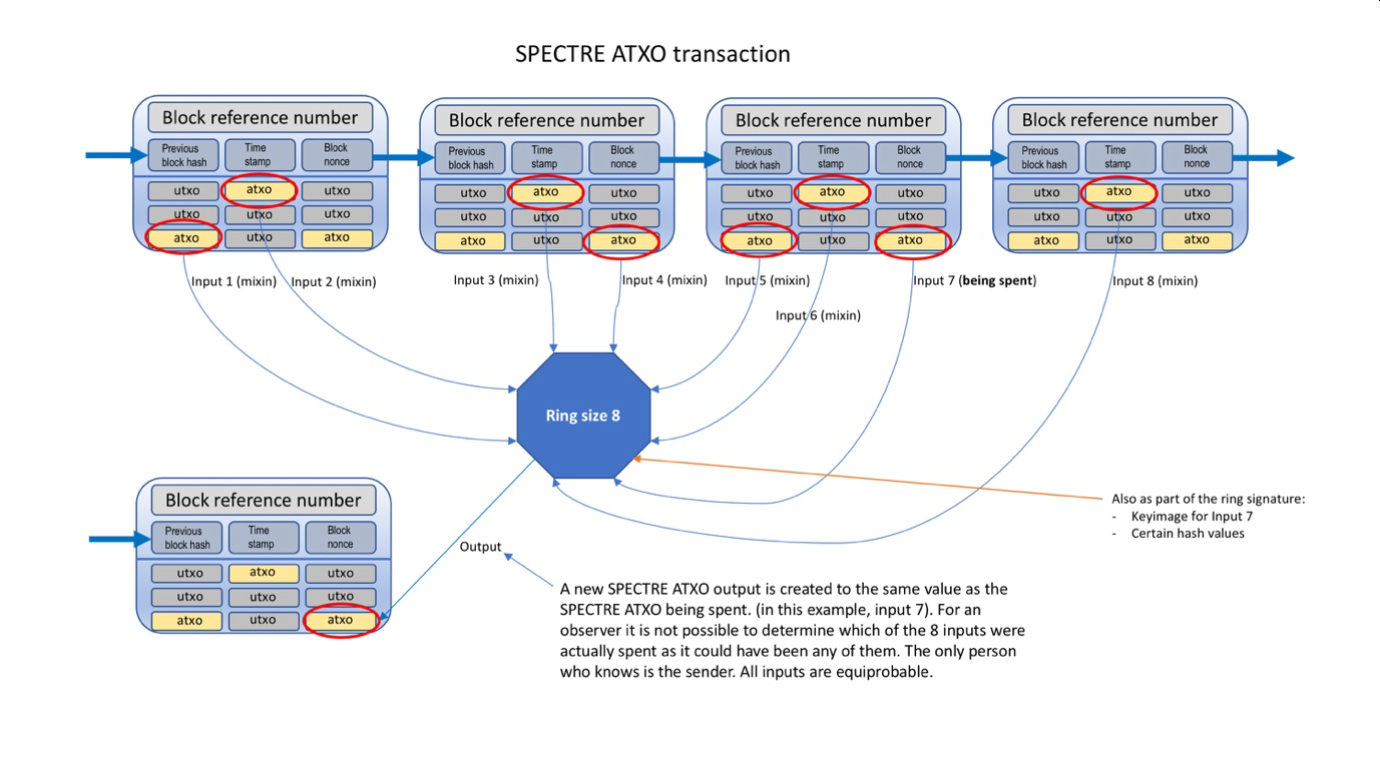
\includegraphics[width=\textwidth]{Anonymous-ATXO-Transaction.png}
\end{figure}



In the Spectrecoin software we talk about ring sizes and this refers to the
group or set of possible signers. So, in the example below, we have a ring
size of 8 which simply means that amongst the 8 public keys that form part
of the digital signature, 7 are so called ‘\textit{mixins}’ or chaff or decoys and
only 1 is the public key corresponding to the SPECTRE being spent. When
conducting an anonymous transaction, we use ring signatures to hide spent
output in a set of the same denomination.



Anonymous transactions in Spectrecoin can be said to have levels of
‘\textit{transactional entropy}’ as there is an interface between the ‘\textit{public}’
and the ‘\textit{anonymous}’ coins. Entropy level 0 can be said to be at the
interface between XSPEC $>>$ SPECTRE and between SPECTRE $>>$ XSPEC. Once
SPECTRE has been created from SPECTRE, i.e. an ATXO used as an input to
create a new ATXO we can say that this is entropy level 1 as the freshly
created ATXO has no public UTXO origin. Once these ATXOs are used to
create further ATXOs this would be entropy level 2 and so on. The entropy
increases with every level, IF AND ONLY IF a minimum ring size is used and
the ATXOs have not been part of any ring size 1 transaction.




\subsection{Minimum Ring Size}

A minimum ring size of 10 is being enforced as part of the consensus since 
Spectrecoin v3.x.



Any ATXO used in a ring size 1 transaction will be marked as 
‘\textit{compromised}’ and will not be selected as a ‘\textit{mixin}’ 
in any future ring signature transaction.



\textbf{We have seen how dual-key stealth address techniques are used to 
create ATXOs on the Spectrecoin blockchain with bundled one-time key pair 
that can only be ‘spent’ by providing a valid ring signature. In this way 
Spectrecoin protects the privacy of both the sender and the receiver.}



\subsection{Ring-Signature formula}
Spectrecoin uses a ring-signature formula developed by Dr. Adam Back. He 
created a formula based on the traceable ring signature described in the 
CryptoNote white-paper\footnote{https://cryptonote.org/whitepaper.pdf} 
using maths based on the paper "\textit{1-out-of-n Signatures from a Variety of Keys}"\footnote{https://www.researchgate.net/publication/221326919\_1-out-of-n\_Signatures\_from\_a\_Variety\_of\_Keys} 
by Abe, Ohkubo and Suzuki. He was able to create a linkable ring signature 
which tends to be \sfrac{1}{2} of the size of the CryptoNote ring signature 
as the signature is 3+n values vs. 2+2n values. 



Dr. A. Back showed how to add traceability in a way that made it compatible with CryptoNote\footnote{https://bitcointalk.org/index.php?topic=972541.msg10619684}. 
The original description contains 4 parts (\textbf{KEYGEN}, \textbf{SIG}, 
\textbf{VERIFY}, \textbf{LINK}) and is summarized here for comparison:


\hfill \break\textbf{Definitions}:
 
\begin{tabular}{ll}
	$q$:   & a prime number; $q = 2^{255} - 19$\\
	$d$:   & an element of $\mathbb{F}_q$;. $-121665/121666$ \\
	$E$:   & an elliptic curve equation; $-x^2 + y^2 = 1 + dx^2y^2$ \\
	$G$:   & a base point; $G=(x, -4/5)$ \\
	$l$:   & a prime order of the base point; $l=2^{252}+27742317777372353535851937790883648493$ \\
	$\mathcal{H}_s$:   & a cryptographic hash function $\{0,1\}^* \rightarrow \mathbb{F}_q$ \\
	$\mathcal{H}_p$:   & a deterministic hash function $E(\mathbb{F}_q) \rightarrow E(\mathbb{F}_q)$ \\	
\end{tabular}

\hfill \break


\hfill \break\textbf{KEYGEN}: 
The signer selects a secret key $x \in [1, l-1]$ and calculates a public 
key $P$, as well as the key-image $I$ with the following equations:

\begin{equation}
\begin{split}
P &= xG\\
I &= x\mathcal{H}_p(P)\\ 
\end{split}
\end{equation}

\textbf{SIG}: 
The signer selects a set $S'$ of $n$ other users public keys $P_i$, and 
adds his own public key to the set. 

\begin{equation}
\begin{split}
S &= S' \cup \{P_s\}\\
 &= \{P_i\}, i \in [0..n] \\
\end{split}
\end{equation}

Note that the public key $P_{i=s}$ is the signer's own public key, while 
the others are random selected public keys that will be used in the ring 
signature. The index $s$ is the signer secret index. The signer then pics 
$n+1$ random private keys $q_i$ and $n$ private keys $w_i$.

\begin{equation}
\begin{split}
q_i &\in [1...l],  i \in [0...n] \\
w_i &\in [1...l],  i \in [0...n], i \not= s \\
\end{split}
\end{equation}

Now he computes:

\[
L_i= 
\begin{dcases}
q_iG,& \text{if } i = s\\
q_iG+w_iP_i,              & \text{otherwise}
\end{dcases}
\]

and similarly

\[
R_i= 
\begin{dcases}
q_i\mathcal{H}_p(P_i),& \text{if } i = s\\
q_i\mathcal{H}_p(P_i)+w_iI,              & \text{otherwise}
\end{dcases}
\]

Now he calculates the challenge $c$:

\begin{equation}
\begin{split}
c &= \mathcal{H}_s(m, L_1, ..., L_n, R_1, ..., R_n)\\
\end{split}
\end{equation}

And finally the response 

\[
c_i= 
\begin{dcases}
w_i,& \text{if } i \not= s\\
c-\sum_{i=0}^n c_i \quad mod\quad l,              & \text{otherwise}
\end{dcases}
\]

and similarly

\[
r_i= 
\begin{dcases}
q_i,& \text{if } i \not= s\\
q_i-c_sx \quad mod\quad l,              & \text{otherwise}
\end{dcases}
\]

The resulting signature $\sigma$ is then
\[
\sigma = (I, c_1, ..., c_n, r_1, ..., r_n)
\]

One can immediatly see that the signature $\sigma$ from the Cryptonote 
whitepaper has $2(n+1)$ values for $c_i$ and $r_i$.

\hfill \break\textbf{VERIFY}: 
The first step is to apply the inverse transformation.

\begin{equation}
\begin{split}
L_i' &= r_iG+c_iP_i\\
R_i' &= r_i*\mathcal{H}_p(P_i)+c_iI\\ 
\end{split}
\end{equation}

A verifier now checks that the following condition holds:

\begin{equation}
\begin{split}
\sum_{i=0}^n c_i &\stackrel{?}{=}	 \mathcal{H}_s(m, L_0', ..., L_n', R_0', R_n')
\end{split}
\end{equation}

\hfill \break\textbf{LINK}: 
This step is only applied when the previous step succeeds. The verifier 
uses a set $\mathcal{I}$ of previous signatures and rejects the signature 
$\sigma = (I,... )$ if $I \in \mathcal{I}$.

\hfill \break Dr. Adam Back's variation, and the version of the ring-signature 
algorithm used by spectrecoin, is as follows:

\hfill \break\textbf{KEYGEN}: Like above, pick a random private key 
$x \in [1..l-1]$ and calculate:

\begin{equation}
\begin{split}
P &= xG\\
I &= x\mathcal{H}_p(P)\\ 
\end{split}
\end{equation}

\hfill \break\textbf{SIG}: Pick $n$ random public keys $P_i$ from other 
users, generate $n$ random private keys $s_i \in [1...l-1]$ as well as a 
private key $\alpha \in [1..l-1]$ for the signer with index $j, 0<=j<=n$. 
This gives you the following structure:

\begin{equation}
\begin{split}
\textbf{public keys} &: [P_0, ... P_j, ..., P_n] \\
\textbf{private keys} &: [s_0, ... s_j, ..., s_n] \\
\end{split}
\end{equation}

\hfill \break NOTE that $s_j$ is to be calculated (see below) and $P_j$ 
is the public key of the signer. The next step is to calculate the parameters 
$c_i$ recursively yielding the vector $[c_0, ... ,c_j, ..., c_n]$.

\begin{equation}
\begin{split}
  c_{j+1} & = \mathcal{H}_s(P_1, ..., P_n, \alpha G, \alpha \mathcal{H}_p(P_j))\\
  c_{j+2} & = \mathcal{H}_s(P_1,...,P_n,s_{j+1}G+c_{j+1}P_{j+1},s_{j+1}\mathcal{H}_p(P_{j+1})+c_{j+1}I_j)\\
	      & ... \\
  c_{j} & = \mathcal{H}_s(P_1,...,P_n,s_{j-1}G+c_{j-1}P_{j-1},s_{j-1}\mathcal{H}_p(P_{j-1})+c_{j-1}I_j) \\
\end{split}
\end{equation}

\hfill \break The formula shows that we start to calculate at the position 
$j+1$ , where $j$ represents the signer's index. To keep the index $i$ of 
$c_i$ within the allowed range, we have to take the $mod$ of the number of 
signers. Effectively we calculate the sequence 
$c_{j+1}, c_{j+2}, ..., c_n, c_0, c_1, ... c_j$
 
\hfill \break Next is to find the $s_j$ value: Adam argues that since 
$\alpha G = s_jG+c_jP_j$ , then $\alpha = s_j+c_jx_j$ or 
$s_j = \alpha - c_jx_j\quad mod\quad n.$

\hfill \break The signature $\sigma$ based on this approach is than given 
by $\sigma = (m,I_j,c_1,s_1,...,s_n)$

\hfill \break\textbf{VERIFY}: 

We compute the following equation $\forall_{i=1..n}$

\begin{equation}
\begin{split}
 e_i &= s_iG+c_iP_i \\
 E_i &= s_i\mathcal{H}_p(P_i)+c_iI_j \\
 c_{i+1} &=\mathcal{H}_s(P_1,...,P_n,e_i,E_i)
\end{split}
\end{equation}

Then we check if $c_{n+1}=c_1$.

\hfill \break\textbf{LINK}: 
Like above, we reject duplicate $I_j$ values.


\hfill \break As we can see from the new signature $\sigma = 
(m,I_j,c_1,s_1,...,s_n)$, this version of the ring signature 
uses only 1/2 of the size of the Cryptonote ring signature.

\subsection{The ‘All\_Spent’ Dilemma}
A ‘\textit{special}‘ situation could occur where all the ATXOs available for a
certain denomination are spent except for your own ATXO to be used in a transaction.
We are referring to this situation as the \textbf{\textit{‘ALL\_SPENT’ dilemma}}
and although this appears to be a very low probability situation in V3 it could
have dire consequences for privacy and compromise a number of ATXOs. Let’s first
explain this dilemma in some detail:



A valid ring signature (\textit{assume ring size 10}) needs: \textbf{(1)} An
unspent ATXO of a certain denomination to be used/spent in the transaction,
and \textbf{(2)} Nine (9) ‘\textit{mixins}’ of the same denomination
(\textit{spent or unspent}). These ‘\textit{mixins}’ (ATXOs) of the same
value as the one being spent provides ‘\textit{plausible deniability}’ with
regards to the sender. The sender could own any one of the ten ATXOs used
in the ring-signature and an observer can not determine which one of the
10 ATXOs forming the ring-signature is being spent. This is at core of
ring-signature privacy and needs to be preserved.



ATXOs of each denomination are “\textit{scattered}” along the Spectrecoin
blockchain and exists in various blocks where they were once created and
they can all be used as ‘\textit{mixins}’ in a ring-signature whether they
have ever been spent or not. Each ATXO is a ‘\textit{unique unit of data}’
identified by its associated ‘\textit{public key}’. However, only the
owner of an ATXO can determine if an ATXO value has been spent or not
as this requires the corresponding ‘\textit{private key}’.



The ATXO picking algorithm for a ring-signature selects 9 ‘\textit{mixins}’
at random from the available pool of ATXOs. In each block there could be a
number of ATXOs of different denominations (\textit{spent or unspent})
that could be selected as the 9 ‘\textit{mixins}’.



Any observer will be able to establish the following: \textbf{(1)} In each
valid ring-signature on the blockchain there will be one and only one ATXO
of a certain denomination being spent. \textbf{(2)} In each valid
ring-signature there will be nine ‘\textit{mixins}’ used of the same
denomination. \textbf{(3)} The observer will be able to count the number
of existing ATXOs for each denomination by scanning the blockchain.
\textbf{(4)} The observer will be able to count the number of ATXOs for
each denomination that has been spent by counting the number of valid
ring-signatures where this denomination has been used.



As a result, if the ‘ALL\_SPENT‘ situation occurs, i.e.:



\textbf{(number\_of\_\_existing\_ATXOs = number\_of\_spent\_ATXOs) }



An observer will be able to categorically determine that each of the ATXOs
used as a ‘\textit{mixin}‘ in the ring-signature has previously been spent.
The sender’s privacy has been compromised as the ‘\textit{real}‘ input ATXO
can be identified, and we no longer have the ‘\textit{plausible deniability}’
afforded by the ring-signature. It is important to point out the following
regarding this issue:



\begin{itemize}
	\item This only occurs when ALL the ATXOs of a denomination have been
	spent and a new transaction is created using the depleted denomination.
	\item The privacy of the transaction spending the last unspent ATXO,
	although creating an ‘ALL\_SPENT‘ situation is not compromised.
	\item If the ‘ALL\_SPENT’ occurs, it would only compromise transaction
	created after the ‘ALL\_SPENT’. All the previous transactions would still
	retain their privacy.
\end{itemize}



\subsubsection{'ALL\_SPENT' illustration}

...

\subsubsection{Solutions}
A range of measures are being implemented to negate the so called
\textit{‘ALL\_SPENT’ dilemma}. We realised that this is only likely
to occur in a situation where there is a very limited supply of
ATXOs of a certain denomination.

Therefore, the main approach to solve this problem is to make sure that
there is always a sufficient supply of ATXOs of varying denominations.
We have therefore introduced an advanced ATXO balancer algorithm. This
algorithm will measure the number of ATXO existing for each denomination
and either seek to consolidate ATXO values or split ATXO values as part
of the staking transaction in PoAS. This will ensure that there are
always sufficient supply of ATXO to act as ‘\textit{mixins}‘.



In addition a new algorithm has been implemented to detect an
‘\textit{ALL\_SPENT}‘ situation and if this situation does occurs
the network will ‘\textit{remember}‘ the block height (\textit{block number})
and the picking algorithm will no longer pick ‘\textit{mixins}‘
from below that block height. This ensures that users get the full
benefit of the privacy the ring-signature offers.



\subsection{The ‘ATXO\_Set’ Dilemma}

We can say that all the ATXOs created in the same transaction are part
of an ‘\textit{ATXO\_Set}’, i.e. they will forever be linked to each
other as they were created at the same time and it can be assumed that
they all belong to the same user. There will always be multiple outputs
per transaction because of the denomination system, because amounts
have to be split into discrete values.



The following dilemma may then occur; the ATXO picking algorithm (as it is
now) could select ATXOs from an ‘\textit{ATXO\_SET}‘ as ‘\textit{mixins}‘
in a ring-signature and this could potentially compromise privacy by making
the signature more susceptible to deductive analysis. In other words, an
observer could be able to determine which of the ‘\textit{mixins}‘ are fake.



\subsubsection{Solutions}
New algorithms have been created to negate these issues and strengthen the
privacy of the network. This way depending on the random pick of the initial
‘\textit{mixins}‘ and the denominations to fill, there will be a random
amount of ‘\textit{mixins}‘ from the same transaction in the final transaction.



This will also ensure that each output is only used once as a ‘\textit{mixin}‘
in one of the ring-signatures (VINs). Something which was previously only
assured by chance. Same ‘\textit{mixin}‘ in different VINs can only be fake.



\begin{itemize}
	\item When the first 9 ‘\textit{mixins}‘ for an output are chosen, it is
	completely random, but is ensured that all ‘\textit{mixins}‘ come from
	different transactions.
	\item When ‘\textit{mixins}‘ for the second ring-signature are chosen,
	there is a 33\% chance that the algorithm tries to 	choose outputs from
	the transaction chosen as ‘\textit{mixins}‘ for the first ring-signature.
	If no outputs can 	picked that way, a new random output is chosen and
	the corresponding transaction is added as new source of ‘\textit{mixins}‘.
	\item Repeat.
\end{itemize}



We believe that these issues also exist in Monero and other CryptoNote based
systems and may have been described first in a paper entitled
\textit{“A Traceability Analysis of Monero’s Blockchain”}
\footnote{https://eprint.iacr.org/2017/338.pdf} and in particular in
chapter: 5.2 Heuristic II: Leveraging Output Merging in this paper.
